\section{Boundary element methods with Bempp}
In this section, we provide a brief introduction to boundary element methods and describe the necessary steps for their numerical discretisation and solution.

The most simple boundary integral equation is of the form
\begin{align}
  \label{eq:bnd_integral}
  \int_{\Gamma} g(\bx, \by)\phi(\by)\,\mathrm{d}s(\by) &= f(\bx),&&\bx\in\Gamma.
\end{align}
The function $g(\bx, \by)$ is a Green's function, $f$ is a given right-hand side, and $\phi$ is an unknown surface density over the boundary $\Gamma$ of a bounded three dimensional domain $\Omega\subset\mathbb{R}^3$.

As a concrete example, we consider computing the electrostatic capacity of an object $\Omega$. In this case, we solve the above equation with $f(\bx)=1$ and $g(\bx,\by)=\frac{1}{4\uppi|\bx - \by|}$. Once $\phi$ has been found, the normalised capacity is then obtained using $c = \frac{1}{4\uppi}\int_{\Gamma}\phi(\bx)\,\mathrm{d}s(\bx)$.

Many practical problems have a significantly more complex structure and can involve block systems of integral equations. Nevertheless, the fundamental structure of what Bempp-cl does is well described by the above problem and will be described in the following.

\begin{figure}
  \centering
  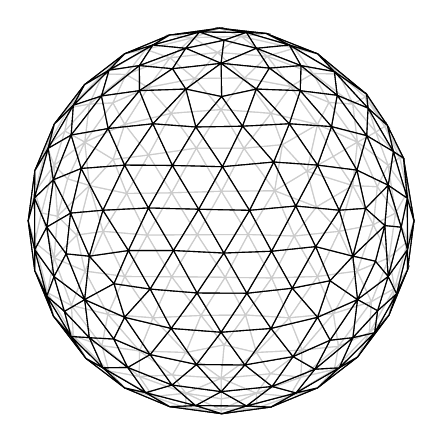
\begin{tikzpicture}[x={(1.732cm,-1cm)},y={(1.732cm,1cm)},z={(0,2cm)}]
\coordinate (v0) at (1.0,0.0,0.0);
\coordinate (v1) at (0.0,1.0,0.0);
\coordinate (v2) at (-1.0,0.0,0.0);
\coordinate (v3) at (0.0,-1.0,0.0);
\coordinate (v4) at (0.0,0.0,-1.0);
\coordinate (v5) at (0.0,0.0,1.0);
\coordinate (v6) at (0.9659258261113405,0.2588190457658098,0.0);
\coordinate (v7) at (0.8660254030594872,0.5000000012556528,0.0);
\coordinate (v8) at (0.7071067795767626,0.7071067827963324,0.0);
\coordinate (v9) at (0.4999999986418108,0.8660254045685896,0.0);
\coordinate (v10) at (0.2588190443111854,0.9659258265011059,0.0);
\coordinate (v11) at (-0.2588190457837957,0.9659258261065212,0.0);
\coordinate (v12) at (-0.5000000013601116,0.8660254029991779,0.0);
\coordinate (v13) at (-0.7071067828732788,0.7071067794998164,0.0);
\coordinate (v14) at (-0.8660254045816592,0.4999999986191735,0.0);
\coordinate (v15) at (-0.9659258264965713,0.258819044328109,0.0);
\coordinate (v16) at (-0.9659258261113405,-0.2588190457658098,0.0);
\coordinate (v17) at (-0.8660254030594872,-0.5000000012556528,0.0);
\coordinate (v18) at (-0.7071067795767626,-0.7071067827963324,0.0);
\coordinate (v19) at (-0.4999999986418108,-0.8660254045685896,0.0);
\coordinate (v20) at (-0.2588190443111854,-0.9659258265011059,0.0);
\coordinate (v21) at (0.2588190457837957,-0.9659258261065212,0.0);
\coordinate (v22) at (0.5000000013601116,-0.8660254029991779,0.0);
\coordinate (v23) at (0.7071067828732788,-0.7071067794998164,0.0);
\coordinate (v24) at (0.8660254045816592,-0.4999999986191735,0.0);
\coordinate (v25) at (0.9659258264965713,-0.258819044328109,0.0);
\coordinate (v26) at (0.0,0.9659258261113405,-0.2588190457658098);
\coordinate (v27) at (0.0,0.8660254030594872,-0.5000000012556528);
\coordinate (v28) at (0.0,0.7071067795767626,-0.7071067827963324);
\coordinate (v29) at (0.0,0.4999999986418108,-0.8660254045685896);
\coordinate (v30) at (0.0,0.2588190443111854,-0.9659258265011059);
\coordinate (v31) at (0.0,-0.2588190457837957,-0.9659258261065212);
\coordinate (v32) at (0.0,-0.5000000013601116,-0.8660254029991779);
\coordinate (v33) at (0.0,-0.7071067828732788,-0.7071067794998164);
\coordinate (v34) at (0.0,-0.8660254045816592,-0.4999999986191735);
\coordinate (v35) at (0.0,-0.9659258264965713,-0.258819044328109);
\coordinate (v36) at (0.0,-0.9659258261113405,0.2588190457658098);
\coordinate (v37) at (0.0,-0.8660254030594872,0.5000000012556528);
\coordinate (v38) at (0.0,-0.7071067795767626,0.7071067827963324);
\coordinate (v39) at (0.0,-0.4999999986418108,0.8660254045685896);
\coordinate (v40) at (0.0,-0.2588190443111854,0.9659258265011059);
\coordinate (v41) at (0.0,0.2588190457837957,0.9659258261065212);
\coordinate (v42) at (0.0,0.5000000013601116,0.8660254029991779);
\coordinate (v43) at (0.0,0.7071067828732788,0.7071067794998164);
\coordinate (v44) at (0.0,0.8660254045816592,0.4999999986191735);
\coordinate (v45) at (0.0,0.9659258264965713,0.258819044328109);
\coordinate (v46) at (0.9659258261113405,0.0,0.2588190457658098);
\coordinate (v47) at (0.8660254030594872,0.0,0.5000000012556528);
\coordinate (v48) at (0.7071067795767626,0.0,0.7071067827963324);
\coordinate (v49) at (0.4999999986418108,0.0,0.8660254045685896);
\coordinate (v50) at (0.2588190443111854,0.0,0.9659258265011059);
\coordinate (v51) at (-0.2588190457837957,0.0,0.9659258261065212);
\coordinate (v52) at (-0.5000000013601116,0.0,0.8660254029991779);
\coordinate (v53) at (-0.7071067828732788,0.0,0.7071067794998164);
\coordinate (v54) at (-0.8660254045816592,0.0,0.4999999986191735);
\coordinate (v55) at (-0.9659258264965713,0.0,0.258819044328109);
\coordinate (v56) at (-0.9659258261113405,0.0,-0.2588190457658098);
\coordinate (v57) at (-0.8660254030594872,0.0,-0.5000000012556528);
\coordinate (v58) at (-0.7071067795767626,0.0,-0.7071067827963324);
\coordinate (v59) at (-0.4999999986418108,0.0,-0.8660254045685896);
\coordinate (v60) at (-0.2588190443111854,0.0,-0.9659258265011059);
\coordinate (v61) at (0.2588190457837957,0.0,-0.9659258261065212);
\coordinate (v62) at (0.5000000013601116,0.0,-0.8660254029991779);
\coordinate (v63) at (0.7071067828732788,0.0,-0.7071067794998164);
\coordinate (v64) at (0.8660254045816592,0.0,-0.4999999986191735);
\coordinate (v65) at (0.9659258264965713,0.0,-0.258819044328109);
\coordinate (v66) at (-0.5968753305573024,0.7703416941999426,0.2243668893204343);
\coordinate (v67) at (-0.25808567630587,0.5868977891779429,0.7674443385243377);
\coordinate (v68) at (-0.7769544900097934,0.2245974601741118,0.5881537104468694);
\coordinate (v69) at (-0.2254249910932218,0.9001119381675856,0.3728385711795151);
\coordinate (v70) at (-0.3787640544764326,0.2205246094336313,0.8988508718213706);
\coordinate (v71) at (-0.9048480989796104,0.3705166486211054,0.2097429924492644);
\coordinate (v72) at (-0.7797560750556357,0.585705630718971,0.2212607189709846);
\coordinate (v73) at (-0.650709021142228,0.6242337603634365,0.4323440025673979);
\coordinate (v74) at (-0.4465168089496794,0.7845299651173139,0.4303022703153183);
\coordinate (v75) at (-0.231240816923478,0.7685299157113522,0.5965875924307369);
\coordinate (v76) at (-0.4739425155526548,0.6200993088613943,0.6251892743080067);
\coordinate (v77) at (-0.6031837146803123,0.2254193786783961,0.7651029255799586);
\coordinate (v78) at (-0.6513658012436212,0.442834451184977,0.6161415158185994);
\coordinate (v79) at (-0.8003871115687095,0.4251399784782245,0.422686045603888);
\coordinate (v80) at (-0.4439412469568365,0.4312895863375229,0.7854490254099811);
\coordinate (v81) at (-0.9039370819570685,0.20705058418685,0.3742357693408044);
\coordinate (v82) at (-0.3877851743099778,0.897240796860791,0.2112038465190635);
\coordinate (v83) at (-0.207731567320233,0.3928339621379274,0.895853933880903);
\coordinate (v84) at (-0.1761804132919844,0.9677027834328927,0.1803386000228983);
\coordinate (v85) at (-0.1685588971098267,0.1898373709799256,0.9672434916327717);
\coordinate (v86) at (-0.9684447980774777,0.1746040072380701,0.1778708464271154);
\coordinate (v87) at (-0.5968753307481794,-0.2243668895376927,0.7703416939887752);
\coordinate (v88) at (-0.2580856747343077,-0.76744433963247,0.5868977884200106);
\coordinate (v89) at (-0.7769544878960637,-0.5881537128406362,0.2245974612176846);
\coordinate (v90) at (-0.2254249911044945,-0.3728385711823959,0.9001119381635698);
\coordinate (v91) at (-0.3787640522362001,-0.89885087303886,0.2205246083185127);
\coordinate (v92) at (-0.904848098645285,-0.2097429941003022,0.3705166485031911);
\coordinate (v93) at (-0.779756075329191,-0.2212607195851551,0.585705630122805);
\coordinate (v94) at (-0.6507090211826841,-0.4323440022848056,0.6242337605170156);
\coordinate (v95) at (-0.4465168096565718,-0.4303022694920272,0.7845299651665554);
\coordinate (v96) at (-0.2312408167647887,-0.5965875924847092,0.7685299157171981);
\coordinate (v97) at (-0.4739425151141017,-0.6251892745748621,0.6200993089275739);
\coordinate (v98) at (-0.6031837130612882,-0.7651029268255582,0.2254193787829455);
\coordinate (v99) at (-0.6513658007101506,-0.6161415159905272,0.4428344517303621);
\coordinate (v100) at (-0.8003871102786878,-0.4226860477315288,0.4251399787912912);
\coordinate (v101) at (-0.4439412449754755,-0.7854490267443461,0.431289585947156);
\coordinate (v102) at (-0.9039370812790738,-0.3742357716630582,0.2070505829492741);
\coordinate (v103) at (-0.3877851738453488,-0.2112038471434982,0.8972407969146465);
\coordinate (v104) at (-0.2077315675057009,-0.8958539340303733,0.3928339616989984);
\coordinate (v105) at (-0.1761804137572365,-0.1803386002115927,0.9677027833130498);
\coordinate (v106) at (-0.1685588964450716,-0.9672434918215602,0.1898373706080592);
\coordinate (v107) at (-0.9684447978110251,-0.1778708478837493,0.1746040072323722);
\coordinate (v108) at (0.2373906267115964,0.5927409723817137,0.7696306924730116);
\coordinate (v109) at (0.7697707710048625,0.5952202488744707,0.2306363113500065);
\coordinate (v110) at (0.7715181150161288,0.2241412011263674,0.5954389220805305);
\coordinate (v111) at (0.2851758031801919,0.9150830133715486,0.2851758031775501);
\coordinate (v112) at (0.3692155676783176,0.2111788235332098,0.905046009811243);
\coordinate (v113) at (0.9150830123989893,0.2851758047394409,0.2851758047394476);
\coordinate (v114) at (0.2753900042236253,0.7911269310737263,0.546175264334329);
\coordinate (v115) at (0.5461752643497462,0.7911269310564869,0.2753900042425727);
\coordinate (v116) at (0.4619648243177169,0.6151122925083028,0.6389312148648023);
\coordinate (v117) at (0.641521731118863,0.6210132027869703,0.4503349340187716);
\coordinate (v118) at (0.8053380981320204,0.4199759472986743,0.4184238142857654);
\coordinate (v119) at (0.5855986155063985,0.2238194347714397,0.7791060214201453);
\coordinate (v120) at (0.63364096670642,0.433732440129488,0.6406140643019629);
\coordinate (v121) at (0.4273171617143365,0.423891712063688,0.7985878884122581);
\coordinate (v122) at (0.2100486925880666,0.3754812074457851,0.9027283031774649);
\coordinate (v123) at (0.4723957159889963,0.7465951543384605,0.4684612272726617);
\coordinate (v124) at (0.1756874204939024,0.1784127050819355,0.9681492048495346);
\coordinate (v125) at (0.8840112368180318,0.1746408047174856,0.4336434724045649);
\coordinate (v126) at (0.8794805302343316,0.4408052756453442,0.1795199461504336);
\coordinate (v127) at (0.9758097728955429,0.1559726491244944,0.1532147208624068);
\coordinate (v128) at (0.1593794995713874,0.9747557310275753,0.1563866823416694);
\coordinate (v129) at (0.1697430886237962,0.8877436557132312,0.4279248189208922);
\coordinate (v130) at (0.4162253125924886,0.8949040748362558,0.1610058480091539);
\coordinate (v131) at (-0.7723547397298042,0.229839038321006,-0.5921735093468681);
\coordinate (v132) at (-0.2319544372565306,0.7681237290935419,-0.5968336483317315);
\coordinate (v133) at (-0.6002447844336112,0.7681146429678114,-0.2230089224107618);
\coordinate (v134) at (-0.3728385711823655,0.2254249911044676,-0.9001119381635893);
\coordinate (v135) at (-0.9029228878282824,0.370193644323789,-0.2184322608026444);
\coordinate (v136) at (-0.2851758047477622,0.9150830123929419,-0.285175804750534);
\coordinate (v137) at (-0.5951954520500858,0.2326861098415221,-0.7691728827103976);
\coordinate (v138) at (-0.4173579798734024,0.4472140676990436,-0.7910989718946118);
\coordinate (v139) at (-0.7741596912071872,0.593014447795586,-0.2214441399507367);
\coordinate (v140) at (-0.6320078110726355,0.634393429350531,-0.4451075820328241);
\coordinate (v141) at (-0.4145091360595434,0.8075628348742852,-0.419586096516264);
\coordinate (v142) at (-0.2232586774497229,0.594825618287681,-0.7722467202843186);
\coordinate (v143) at (-0.442027272315798,0.6402729051141058,-0.6282297000268782);
\coordinate (v144) at (-0.901036262032701,0.2082665060571496,-0.3805044601932027);
\coordinate (v145) at (-0.7924702203401054,0.4297451505211725,-0.432823142783372);
\coordinate (v146) at (-0.6295156876644074,0.4543634859921001,-0.6302954482419656);
\coordinate (v147) at (-0.2096366631826169,0.3885403959646253,-0.8972815223758099);
\coordinate (v148) at (-0.9675893252358235,0.1758101501409081,-0.1813062535139228);
\coordinate (v149) at (-0.1680732355016323,0.1901950459158499,-0.967257730977304);
\coordinate (v150) at (-0.4336434737700136,0.8840112359203006,-0.1746408058717195);
\coordinate (v151) at (-0.1795199467464361,0.8794805300870903,-0.4408052756964803);
\coordinate (v152) at (-0.1532147209534412,0.9758097728748019,-0.1559726491648589);
\coordinate (v153) at (0.7657229958867138,0.6013042679501603,-0.2283168825477369);
\coordinate (v154) at (0.5877361365262779,0.2433726647591427,-0.7715982068018842);
\coordinate (v155) at (0.2254250129109098,0.7729438626059109,-0.5931006882585448);
\coordinate (v156) at (0.2176133561645956,0.3768755103605308,-0.9003527756399743);
\coordinate (v157) at (0.9001119381675905,0.2254249910932214,-0.3728385711795036);
\coordinate (v158) at (0.3787932747739996,0.901003975299685,-0.2115011355874853);
\coordinate (v159) at (0.5970339286614769,0.7725015625867129,-0.2163755122369979);
\coordinate (v160) at (0.6296043507869505,0.6434769922698669,-0.4353695214622952);
\coordinate (v161) at (0.768534062862255,0.2316585676444229,-0.5964201733242775);
\coordinate (v162) at (0.778859096757814,0.4518873813342889,-0.4349711884265977);
\coordinate (v163) at (0.6247354038022158,0.4619833128771551,-0.6295115010417719);
\coordinate (v164) at (0.23011863963793,0.5938356425391235,-0.770994116454625);
\coordinate (v165) at (0.4539570255996985,0.6487224386308964,-0.610811776273649);
\coordinate (v166) at (0.4347529553598408,0.4265616777137352,-0.7931336139907178);
\coordinate (v167) at (0.8964021109005491,0.3901819199384114,-0.2103491058737358);
\coordinate (v168) at (0.2128691406017332,0.9041562549852469,-0.3704231790863897);
\coordinate (v169) at (0.3853300004172362,0.2002884393565442,-0.9007938010718928);
\coordinate (v170) at (0.4335697012091362,0.798906198245832,-0.4168849084349718);
\coordinate (v171) at (0.1782009565922777,0.9677655603522645,-0.1780012466421906);
\coordinate (v172) at (0.9677538119750918,0.1795483917067467,-0.1767063714688659);
\coordinate (v173) at (0.1861291197390319,0.1763154172173644,-0.9665813403316981);
\coordinate (v174) at (-0.7704943006792206,-0.59710982040261,-0.2232158618824846);
\coordinate (v175) at (-0.2287168084391019,-0.5942629460650517,-0.771081962482446);
\coordinate (v176) at (-0.7729438626060494,-0.225425012911137,-0.5931006882582779);
\coordinate (v177) at (-0.3752955595818615,-0.901719900955972,-0.2146623967663249);
\coordinate (v178) at (-0.372838571182401,-0.225424991104492,-0.9001119381635685);
\coordinate (v179) at (-0.9150830123990066,-0.2851758047394184,-0.2851758047394148);
\coordinate (v180) at (-0.2151766899186381,-0.7754770001747973,-0.5935999542172238);
\coordinate (v181) at (-0.4368242221604006,-0.6471083226696589,-0.624856926085817);
\coordinate (v182) at (-0.4302556048369856,-0.4440037382365219,-0.7859806576517545);
\coordinate (v183) at (-0.5916150920544347,-0.239218380891727,-0.7699310318190187);
\coordinate (v184) at (-0.6308909327668567,-0.467733352975124,-0.619038883742423);
\coordinate (v185) at (-0.614587983026649,-0.6583496721760371,-0.4345901167994557);
\coordinate (v186) at (-0.8003097539065411,-0.4244380019930233,-0.4235371190648015);
\coordinate (v187) at (-0.4301369881804004,-0.7985152788615917,-0.4211677476646139);
\coordinate (v188) at (-0.5898880121883503,-0.776309387782573,-0.2222674340304155);
\coordinate (v189) at (-0.207731568497199,-0.3928339599670561,-0.8958539345599623);
\coordinate (v190) at (-0.1945517472087195,-0.9048553530467243,-0.3786946864308662);
\coordinate (v191) at (-0.1665780690137853,-0.1906387578805186,-0.9674289659956561);
\coordinate (v192) at (-0.1829409767921664,-0.9659672615242203,-0.1828955625390885);
\coordinate (v193) at (-0.8840112364740983,-0.4336434729242771,-0.1746408051681598);
\coordinate (v194) at (-0.8794805301669909,-0.1795199464211402,-0.4408052756694942);
\coordinate (v195) at (-0.9777920893726778,-0.1482194832423213,-0.1481882527629938);
\coordinate (v196) at (0.5951141306623251,-0.771360998253499,0.2255403394742468);
\coordinate (v197) at (0.2381722620478427,-0.5946827086731585,0.7678893295261325);
\coordinate (v198) at (0.7729438626064933,-0.2254250129110194,0.5931006882577443);
\coordinate (v199) at (0.9006206293770568,-0.3792903710026838,0.2122419166035303);
\coordinate (v200) at (0.2216723266252707,-0.9010051593762881,0.3729306002560798);
\coordinate (v201) at (0.377385998800413,-0.2201314083408526,0.8995265939060715);
\coordinate (v202) at (0.7772952789028376,-0.5882493438695642,0.2231630972496919);
\coordinate (v203) at (0.6474011490719067,-0.6270641183472476,0.4332130496658635);
\coordinate (v204) at (0.440977913386104,-0.7894918225741926,0.426926817450477);
\coordinate (v205) at (0.2402400413445714,-0.772542691726231,0.5877841768107366);
\coordinate (v206) at (0.4661174811643206,-0.6298251331439748,0.6213388486980316);
\coordinate (v207) at (0.595225348782834,-0.2097679201944678,0.7757127801797813);
\coordinate (v208) at (0.6521231806588578,-0.4440157397006633,0.6144879067302715);
\coordinate (v209) at (0.7989720496143149,-0.4292442929488189,0.421212320174436);
\coordinate (v210) at (0.4447569681669115,-0.4345957936598091,0.7831615818717098);
\coordinate (v211) at (0.8983430246080711,-0.205350738490668,0.3883757159412087);
\coordinate (v212) at (0.3812201894375025,-0.9008125066074991,0.2079252372165344);
\coordinate (v213) at (0.2077315664595707,-0.3928339595673662,0.8958539352075814);
\coordinate (v214) at (0.1823438369838656,-0.9673803970286905,0.1758870196407169);
\coordinate (v215) at (0.1805379416169278,-0.1767900139325556,0.9675544582965597);
\coordinate (v216) at (0.9675706945928364,-0.168717838984903,0.1880197601956982);
\coordinate (v217) at (0.5921735102805579,-0.7723547387630713,-0.2298390391640635);
\coordinate (v218) at (0.5968336480630774,-0.2319544371327693,-0.7681237293396584);
\coordinate (v219) at (0.2230089222143883,-0.600244784428311,-0.7681146430289603);
\coordinate (v220) at (0.9001119381676049,-0.3728385711794845,-0.2254249910931948);
\coordinate (v221) at (0.2184322608156712,-0.9029228876954322,-0.3701936446401466);
\coordinate (v222) at (0.2851758047588487,-0.2851758047588553,-0.915083012386894);
\coordinate (v223) at (0.76917288303696,-0.5951954515395242,-0.2326861100680429);
\coordinate (v224) at (0.7910989719184124,-0.4173579809643789,-0.4472140666387888);
\coordinate (v225) at (0.7722467196839322,-0.2232586794706518,-0.5948256183087112);
\coordinate (v226) at (0.2214441399410167,-0.7741596911311408,-0.5930144478984903);
\coordinate (v227) at (0.4451075823207684,-0.6320078102297472,-0.634393429988193);
\coordinate (v228) at (0.4195860962526905,-0.4145091359583019,-0.807562835063212);
\coordinate (v229) at (0.6282296993668646,-0.4420272719032937,-0.6402729060465315);
\coordinate (v230) at (0.3805044610945562,-0.9010362615995603,-0.2082665062844167);
\coordinate (v231) at (0.4328231441734263,-0.7924702192301187,-0.4297451511678274);
\coordinate (v232) at (0.6302954480652208,-0.6295156872519587,-0.4543634868086169);
\coordinate (v233) at (0.8972815220942609,-0.2096366637355367,-0.3885403963165883);
\coordinate (v234) at (0.1813062540696644,-0.967589325093164,-0.1758101503530989);
\coordinate (v235) at (0.9672577307597976,-0.1680732363709023,-0.1901950462540888);
\coordinate (v236) at (0.1746408041726567,-0.4336434718144752,-0.884011237215081);
\coordinate (v237) at (0.4408052757569241,-0.1795199468247579,-0.8794805300408145);
\coordinate (v238) at (0.1559726507051513,-0.1532147206022448,-0.9758097726837831);
\draw[fill=white, fill opacity=0.8] (v143) -- (v146) -- (v140) -- cycle;
\draw[fill=white, fill opacity=0.8] (v140) -- (v146) -- (v145) -- cycle;
\draw[fill=white, fill opacity=0.8] (v138) -- (v146) -- (v143) -- cycle;
\draw[fill=white, fill opacity=0.8] (v141) -- (v143) -- (v140) -- cycle;
\draw[fill=white, fill opacity=0.8] (v137) -- (v146) -- (v138) -- cycle;
\draw[fill=white, fill opacity=0.8] (v145) -- (v146) -- (v131) -- cycle;
\draw[fill=white, fill opacity=0.8] (v138) -- (v143) -- (v142) -- cycle;
\draw[fill=white, fill opacity=0.8] (v140) -- (v145) -- (v139) -- cycle;
\draw[fill=white, fill opacity=0.8] (v132) -- (v143) -- (v141) -- cycle;
\draw[fill=white, fill opacity=0.8] (v133) -- (v141) -- (v140) -- cycle;
\draw[fill=white, fill opacity=0.8] (v131) -- (v146) -- (v137) -- cycle;
\draw[fill=white, fill opacity=0.8] (v142) -- (v143) -- (v132) -- cycle;
\draw[fill=white, fill opacity=0.8] (v133) -- (v140) -- (v139) -- cycle;
\draw[fill=white, fill opacity=0.8] (v137) -- (v138) -- (v134) -- cycle;
\draw[fill=white, fill opacity=0.8] (v142) -- (v147) -- (v138) -- cycle;
\draw[fill=white, fill opacity=0.8] (v144) -- (v145) -- (v131) -- cycle;
\draw[fill=white, fill opacity=0.8] (v141) -- (v151) -- (v132) -- cycle;
\draw[fill=white, fill opacity=0.8] (v139) -- (v145) -- (v135) -- cycle;
\draw[fill=white, fill opacity=0.8] (v133) -- (v150) -- (v141) -- cycle;
\draw[fill=white, fill opacity=0.8] (v138) -- (v147) -- (v134) -- cycle;
\draw[fill=white, fill opacity=0.8] (v135) -- (v145) -- (v144) -- cycle;
\draw[fill=white, fill opacity=0.8] (v136) -- (v151) -- (v141) -- cycle;
\draw[fill=white, fill opacity=0.8] (v141) -- (v150) -- (v136) -- cycle;
\draw[fill=white, fill opacity=0.8] (v131) -- (v137) -- (v58) -- cycle;
\draw[fill=white, fill opacity=0.8] (v28) -- (v142) -- (v132) -- cycle;
\draw[fill=white, fill opacity=0.8] (v133) -- (v139) -- (v13) -- cycle;
\draw[fill=white, fill opacity=0.8] (v132) -- (v151) -- (v27) -- cycle;
\draw[fill=white, fill opacity=0.8] (v59) -- (v137) -- (v134) -- cycle;
\draw[fill=white, fill opacity=0.8] (v29) -- (v147) -- (v142) -- cycle;
\draw[fill=white, fill opacity=0.8] (v57) -- (v144) -- (v131) -- cycle;
\draw[fill=white, fill opacity=0.8] (v12) -- (v150) -- (v133) -- cycle;
\draw[fill=white, fill opacity=0.8] (v14) -- (v139) -- (v135) -- cycle;
\draw[fill=white, fill opacity=0.8] (v58) -- (v137) -- (v59) -- cycle;
\draw[fill=white, fill opacity=0.8] (v28) -- (v132) -- (v27) -- cycle;
\draw[fill=white, fill opacity=0.8] (v57) -- (v131) -- (v58) -- cycle;
\draw[fill=white, fill opacity=0.8] (v12) -- (v133) -- (v13) -- cycle;
\draw[fill=white, fill opacity=0.8] (v29) -- (v142) -- (v28) -- cycle;
\draw[fill=white, fill opacity=0.8] (v13) -- (v139) -- (v14) -- cycle;
\draw[fill=white, fill opacity=0.8] (v147) -- (v149) -- (v134) -- cycle;
\draw[fill=white, fill opacity=0.8] (v144) -- (v148) -- (v135) -- cycle;
\draw[fill=white, fill opacity=0.8] (v26) -- (v151) -- (v136) -- cycle;
\draw[fill=white, fill opacity=0.8] (v136) -- (v150) -- (v11) -- cycle;
\draw[fill=white, fill opacity=0.8] (v27) -- (v151) -- (v26) -- cycle;
\draw[fill=white, fill opacity=0.8] (v59) -- (v134) -- (v60) -- cycle;
\draw[fill=white, fill opacity=0.8] (v30) -- (v147) -- (v29) -- cycle;
\draw[fill=white, fill opacity=0.8] (v11) -- (v150) -- (v12) -- cycle;
\draw[fill=white, fill opacity=0.8] (v14) -- (v135) -- (v15) -- cycle;
\draw[fill=white, fill opacity=0.8] (v56) -- (v144) -- (v57) -- cycle;
\draw[fill=white, fill opacity=0.8] (v134) -- (v149) -- (v60) -- cycle;
\draw[fill=white, fill opacity=0.8] (v30) -- (v149) -- (v147) -- cycle;
\draw[fill=white, fill opacity=0.8] (v135) -- (v148) -- (v15) -- cycle;
\draw[fill=white, fill opacity=0.8] (v56) -- (v148) -- (v144) -- cycle;
\draw[fill=white, fill opacity=0.8] (v11) -- (v152) -- (v136) -- cycle;
\draw[fill=white, fill opacity=0.8] (v136) -- (v152) -- (v26) -- cycle;
\draw[fill=white, fill opacity=0.8] (v14) -- (v72) -- (v13) -- cycle;
\draw[fill=white, fill opacity=0.8] (v13) -- (v66) -- (v12) -- cycle;
\draw[fill=white, fill opacity=0.8] (v27) -- (v155) -- (v28) -- cycle;
\draw[fill=white, fill opacity=0.8] (v58) -- (v176) -- (v57) -- cycle;
\draw[fill=white, fill opacity=0.8] (v28) -- (v164) -- (v29) -- cycle;
\draw[fill=white, fill opacity=0.8] (v59) -- (v183) -- (v58) -- cycle;
\draw[fill=white, fill opacity=0.8] (v57) -- (v194) -- (v56) -- cycle;
\draw[fill=white, fill opacity=0.8] (v13) -- (v72) -- (v66) -- cycle;
\draw[fill=white, fill opacity=0.8] (v155) -- (v164) -- (v28) -- cycle;
\draw[fill=white, fill opacity=0.8] (v58) -- (v183) -- (v176) -- cycle;
\draw[fill=white, fill opacity=0.8] (v12) -- (v82) -- (v11) -- cycle;
\draw[fill=white, fill opacity=0.8] (v15) -- (v71) -- (v14) -- cycle;
\draw[fill=white, fill opacity=0.8] (v26) -- (v168) -- (v27) -- cycle;
\draw[fill=white, fill opacity=0.8] (v29) -- (v156) -- (v30) -- cycle;
\draw[fill=white, fill opacity=0.8] (v176) -- (v194) -- (v57) -- cycle;
\draw[fill=white, fill opacity=0.8] (v60) -- (v178) -- (v59) -- cycle;
\draw[fill=white, fill opacity=0.8] (v66) -- (v82) -- (v12) -- cycle;
\draw[fill=white, fill opacity=0.8] (v71) -- (v72) -- (v14) -- cycle;
\draw[fill=white, fill opacity=0.8] (v27) -- (v168) -- (v155) -- cycle;
\draw[fill=white, fill opacity=0.8] (v29) -- (v164) -- (v156) -- cycle;
\draw[fill=white, fill opacity=0.8] (v4) -- (v149) -- (v30) -- cycle;
\draw[fill=white, fill opacity=0.8] (v60) -- (v149) -- (v4) -- cycle;
\draw[fill=white, fill opacity=0.8] (v2) -- (v148) -- (v56) -- cycle;
\draw[fill=white, fill opacity=0.8] (v15) -- (v148) -- (v2) -- cycle;
\draw[fill=white, fill opacity=0.8] (v178) -- (v183) -- (v59) -- cycle;
\draw[fill=white, fill opacity=0.8] (v1) -- (v152) -- (v11) -- cycle;
\draw[fill=white, fill opacity=0.8] (v26) -- (v152) -- (v1) -- cycle;
\draw[fill=white, fill opacity=0.8] (v56) -- (v194) -- (v179) -- cycle;
\draw[fill=white, fill opacity=0.8] (v82) -- (v84) -- (v11) -- cycle;
\draw[fill=white, fill opacity=0.8] (v15) -- (v86) -- (v71) -- cycle;
\draw[fill=white, fill opacity=0.8] (v26) -- (v171) -- (v168) -- cycle;
\draw[fill=white, fill opacity=0.8] (v156) -- (v173) -- (v30) -- cycle;
\draw[fill=white, fill opacity=0.8] (v60) -- (v191) -- (v178) -- cycle;
\draw[fill=white, fill opacity=0.8] (v56) -- (v195) -- (v2) -- cycle;
\draw[fill=white, fill opacity=0.8] (v1) -- (v171) -- (v26) -- cycle;
\draw[fill=white, fill opacity=0.8] (v2) -- (v86) -- (v15) -- cycle;
\draw[fill=white, fill opacity=0.8] (v11) -- (v84) -- (v1) -- cycle;
\draw[fill=white, fill opacity=0.8] (v30) -- (v173) -- (v4) -- cycle;
\draw[fill=white, fill opacity=0.8] (v4) -- (v191) -- (v60) -- cycle;
\draw[fill=white, fill opacity=0.8] (v72) -- (v73) -- (v66) -- cycle;
\draw[fill=white, fill opacity=0.8] (v179) -- (v195) -- (v56) -- cycle;
\draw[fill=white, fill opacity=0.8] (v155) -- (v165) -- (v164) -- cycle;
\draw[fill=white, fill opacity=0.8] (v186) -- (v194) -- (v176) -- cycle;
\draw[fill=white, fill opacity=0.8] (v183) -- (v184) -- (v176) -- cycle;
\draw[fill=white, fill opacity=0.8] (v74) -- (v82) -- (v66) -- cycle;
\draw[fill=white, fill opacity=0.8] (v71) -- (v79) -- (v72) -- cycle;
\draw[fill=white, fill opacity=0.8] (v168) -- (v170) -- (v155) -- cycle;
\draw[fill=white, fill opacity=0.8] (v164) -- (v166) -- (v156) -- cycle;
\draw[fill=white, fill opacity=0.8] (v182) -- (v183) -- (v178) -- cycle;
\draw[fill=white, fill opacity=0.8] (v179) -- (v194) -- (v186) -- cycle;
\draw[fill=white, fill opacity=0.8] (v69) -- (v84) -- (v82) -- cycle;
\draw[fill=white, fill opacity=0.8] (v72) -- (v79) -- (v73) -- cycle;
\draw[fill=white, fill opacity=0.8] (v73) -- (v74) -- (v66) -- cycle;
\draw[fill=white, fill opacity=0.8] (v71) -- (v86) -- (v81) -- cycle;
\draw[fill=white, fill opacity=0.8] (v168) -- (v171) -- (v158) -- cycle;
\draw[fill=white, fill opacity=0.8] (v169) -- (v173) -- (v156) -- cycle;
\draw[fill=white, fill opacity=0.8] (v155) -- (v170) -- (v165) -- cycle;
\draw[fill=white, fill opacity=0.8] (v165) -- (v166) -- (v164) -- cycle;
\draw[fill=white, fill opacity=0.8] (v184) -- (v186) -- (v176) -- cycle;
\draw[fill=white, fill opacity=0.8] (v178) -- (v191) -- (v189) -- cycle;
\draw[fill=white, fill opacity=0.8] (v2) -- (v195) -- (v16) -- cycle;
\draw[fill=white, fill opacity=0.8] (v182) -- (v184) -- (v183) -- cycle;
\draw[fill=white, fill opacity=0.8] (v10) -- (v171) -- (v1) -- cycle;
\draw[fill=white, fill opacity=0.8] (v55) -- (v86) -- (v2) -- cycle;
\draw[fill=white, fill opacity=0.8] (v1) -- (v84) -- (v45) -- cycle;
\draw[fill=white, fill opacity=0.8] (v4) -- (v173) -- (v61) -- cycle;
\draw[fill=white, fill opacity=0.8] (v31) -- (v191) -- (v4) -- cycle;
\draw[fill=white, fill opacity=0.8] (v69) -- (v82) -- (v74) -- cycle;
\draw[fill=white, fill opacity=0.8] (v71) -- (v81) -- (v79) -- cycle;
\draw[fill=white, fill opacity=0.8] (v16) -- (v195) -- (v179) -- cycle;
\draw[fill=white, fill opacity=0.8] (v158) -- (v170) -- (v168) -- cycle;
\draw[fill=white, fill opacity=0.8] (v166) -- (v169) -- (v156) -- cycle;
\draw[fill=white, fill opacity=0.8] (v178) -- (v189) -- (v182) -- cycle;
\draw[fill=white, fill opacity=0.8] (v45) -- (v84) -- (v69) -- cycle;
\draw[fill=white, fill opacity=0.8] (v81) -- (v86) -- (v55) -- cycle;
\draw[fill=white, fill opacity=0.8] (v158) -- (v171) -- (v10) -- cycle;
\draw[fill=white, fill opacity=0.8] (v61) -- (v173) -- (v169) -- cycle;
\draw[fill=white, fill opacity=0.8] (v61) -- (v238) -- (v4) -- cycle;
\draw[fill=white, fill opacity=0.8] (v4) -- (v238) -- (v31) -- cycle;
\draw[fill=white, fill opacity=0.8] (v1) -- (v128) -- (v10) -- cycle;
\draw[fill=white, fill opacity=0.8] (v45) -- (v128) -- (v1) -- cycle;
\draw[fill=white, fill opacity=0.8] (v189) -- (v191) -- (v31) -- cycle;
\draw[fill=white, fill opacity=0.8] (v186) -- (v193) -- (v179) -- cycle;
\draw[fill=white, fill opacity=0.8] (v2) -- (v107) -- (v55) -- cycle;
\draw[fill=white, fill opacity=0.8] (v16) -- (v107) -- (v2) -- cycle;
\draw[fill=white, fill opacity=0.8] (v179) -- (v193) -- (v16) -- cycle;
\draw[fill=white, fill opacity=0.8] (v73) -- (v79) -- (v78) -- cycle;
\draw[fill=white, fill opacity=0.8] (v73) -- (v76) -- (v74) -- cycle;
\draw[fill=white, fill opacity=0.8] (v163) -- (v166) -- (v165) -- cycle;
\draw[fill=white, fill opacity=0.8] (v165) -- (v170) -- (v160) -- cycle;
\draw[fill=white, fill opacity=0.8] (v185) -- (v186) -- (v184) -- cycle;
\draw[fill=white, fill opacity=0.8] (v181) -- (v184) -- (v182) -- cycle;
\draw[fill=white, fill opacity=0.8] (v74) -- (v75) -- (v69) -- cycle;
\draw[fill=white, fill opacity=0.8] (v79) -- (v81) -- (v68) -- cycle;
\draw[fill=white, fill opacity=0.8] (v154) -- (v169) -- (v166) -- cycle;
\draw[fill=white, fill opacity=0.8] (v159) -- (v170) -- (v158) -- cycle;
\draw[fill=white, fill opacity=0.8] (v182) -- (v189) -- (v175) -- cycle;
\draw[fill=white, fill opacity=0.8] (v45) -- (v69) -- (v44) -- cycle;
\draw[fill=white, fill opacity=0.8] (v174) -- (v193) -- (v186) -- cycle;
\draw[fill=white, fill opacity=0.8] (v54) -- (v81) -- (v55) -- cycle;
\draw[fill=white, fill opacity=0.8] (v9) -- (v158) -- (v10) -- cycle;
\draw[fill=white, fill opacity=0.8] (v73) -- (v78) -- (v76) -- cycle;
\draw[fill=white, fill opacity=0.8] (v61) -- (v169) -- (v62) -- cycle;
\draw[fill=white, fill opacity=0.8] (v32) -- (v189) -- (v31) -- cycle;
\draw[fill=white, fill opacity=0.8] (v163) -- (v165) -- (v160) -- cycle;
\draw[fill=white, fill opacity=0.8] (v31) -- (v238) -- (v222) -- cycle;
\draw[fill=white, fill opacity=0.8] (v222) -- (v238) -- (v61) -- cycle;
\draw[fill=white, fill opacity=0.8] (v16) -- (v193) -- (v17) -- cycle;
\draw[fill=white, fill opacity=0.8] (v78) -- (v79) -- (v68) -- cycle;
\draw[fill=white, fill opacity=0.8] (v128) -- (v130) -- (v10) -- cycle;
\draw[fill=white, fill opacity=0.8] (v154) -- (v166) -- (v163) -- cycle;
\draw[fill=white, fill opacity=0.8] (v74) -- (v76) -- (v75) -- cycle;
\draw[fill=white, fill opacity=0.8] (v45) -- (v129) -- (v128) -- cycle;
\draw[fill=white, fill opacity=0.8] (v55) -- (v107) -- (v92) -- cycle;
\draw[fill=white, fill opacity=0.8] (v102) -- (v107) -- (v16) -- cycle;
\draw[fill=white, fill opacity=0.8] (v160) -- (v170) -- (v159) -- cycle;
\draw[fill=white, fill opacity=0.8] (v181) -- (v182) -- (v175) -- cycle;
\draw[fill=white, fill opacity=0.8] (v181) -- (v185) -- (v184) -- cycle;
\draw[fill=white, fill opacity=0.8] (v174) -- (v186) -- (v185) -- cycle;
\draw[fill=white, fill opacity=0.8] (v69) -- (v75) -- (v44) -- cycle;
\draw[fill=white, fill opacity=0.8] (v68) -- (v81) -- (v54) -- cycle;
\draw[fill=white, fill opacity=0.8] (v62) -- (v169) -- (v154) -- cycle;
\draw[fill=white, fill opacity=0.8] (v9) -- (v159) -- (v158) -- cycle;
\draw[fill=white, fill opacity=0.8] (v175) -- (v189) -- (v32) -- cycle;
\draw[fill=white, fill opacity=0.8] (v55) -- (v92) -- (v54) -- cycle;
\draw[fill=white, fill opacity=0.8] (v17) -- (v102) -- (v16) -- cycle;
\draw[fill=white, fill opacity=0.8] (v10) -- (v130) -- (v9) -- cycle;
\draw[fill=white, fill opacity=0.8] (v17) -- (v193) -- (v174) -- cycle;
\draw[fill=white, fill opacity=0.8] (v44) -- (v129) -- (v45) -- cycle;
\draw[fill=white, fill opacity=0.8] (v31) -- (v236) -- (v32) -- cycle;
\draw[fill=white, fill opacity=0.8] (v62) -- (v237) -- (v61) -- cycle;
\draw[fill=white, fill opacity=0.8] (v222) -- (v236) -- (v31) -- cycle;
\draw[fill=white, fill opacity=0.8] (v111) -- (v130) -- (v128) -- cycle;
\draw[fill=white, fill opacity=0.8] (v61) -- (v237) -- (v222) -- cycle;
\draw[fill=white, fill opacity=0.8] (v128) -- (v129) -- (v111) -- cycle;
\draw[fill=white, fill opacity=0.8] (v92) -- (v107) -- (v102) -- cycle;
\draw[fill=white, fill opacity=0.8] (v78) -- (v80) -- (v76) -- cycle;
\draw[fill=white, fill opacity=0.8] (v162) -- (v163) -- (v160) -- cycle;
\draw[fill=white, fill opacity=0.8] (v77) -- (v78) -- (v68) -- cycle;
\draw[fill=white, fill opacity=0.8] (v154) -- (v163) -- (v161) -- cycle;
\draw[fill=white, fill opacity=0.8] (v75) -- (v76) -- (v67) -- cycle;
\draw[fill=white, fill opacity=0.8] (v153) -- (v160) -- (v159) -- cycle;
\draw[fill=white, fill opacity=0.8] (v181) -- (v187) -- (v185) -- cycle;
\draw[fill=white, fill opacity=0.8] (v180) -- (v181) -- (v175) -- cycle;
\draw[fill=white, fill opacity=0.8] (v185) -- (v188) -- (v174) -- cycle;
\draw[fill=white, fill opacity=0.8] (v62) -- (v154) -- (v63) -- cycle;
\draw[fill=white, fill opacity=0.8] (v53) -- (v68) -- (v54) -- cycle;
\draw[fill=white, fill opacity=0.8] (v33) -- (v175) -- (v32) -- cycle;
\draw[fill=white, fill opacity=0.8] (v44) -- (v75) -- (v43) -- cycle;
\draw[fill=white, fill opacity=0.8] (v17) -- (v174) -- (v18) -- cycle;
\draw[fill=white, fill opacity=0.8] (v8) -- (v159) -- (v9) -- cycle;
\draw[fill=white, fill opacity=0.8] (v92) -- (v93) -- (v54) -- cycle;
\draw[fill=white, fill opacity=0.8] (v9) -- (v130) -- (v115) -- cycle;
\draw[fill=white, fill opacity=0.8] (v89) -- (v102) -- (v17) -- cycle;
\draw[fill=white, fill opacity=0.8] (v76) -- (v80) -- (v67) -- cycle;
\draw[fill=white, fill opacity=0.8] (v161) -- (v163) -- (v162) -- cycle;
\draw[fill=white, fill opacity=0.8] (v115) -- (v130) -- (v111) -- cycle;
\draw[fill=white, fill opacity=0.8] (v77) -- (v80) -- (v78) -- cycle;
\draw[fill=white, fill opacity=0.8] (v114) -- (v129) -- (v44) -- cycle;
\draw[fill=white, fill opacity=0.8] (v153) -- (v162) -- (v160) -- cycle;
\draw[fill=white, fill opacity=0.8] (v111) -- (v129) -- (v114) -- cycle;
\draw[fill=white, fill opacity=0.8] (v92) -- (v102) -- (v100) -- cycle;
\draw[fill=white, fill opacity=0.8] (v228) -- (v236) -- (v222) -- cycle;
\draw[fill=white, fill opacity=0.8] (v32) -- (v236) -- (v219) -- cycle;
\draw[fill=white, fill opacity=0.8] (v222) -- (v237) -- (v228) -- cycle;
\draw[fill=white, fill opacity=0.8] (v218) -- (v237) -- (v62) -- cycle;
\draw[fill=white, fill opacity=0.8] (v180) -- (v187) -- (v181) -- cycle;
\draw[fill=white, fill opacity=0.8] (v154) -- (v161) -- (v63) -- cycle;
\draw[fill=white, fill opacity=0.8] (v43) -- (v75) -- (v67) -- cycle;
\draw[fill=white, fill opacity=0.8] (v187) -- (v188) -- (v185) -- cycle;
\draw[fill=white, fill opacity=0.8] (v53) -- (v77) -- (v68) -- cycle;
\draw[fill=white, fill opacity=0.8] (v153) -- (v159) -- (v8) -- cycle;
\draw[fill=white, fill opacity=0.8] (v33) -- (v180) -- (v175) -- cycle;
\draw[fill=white, fill opacity=0.8] (v174) -- (v188) -- (v18) -- cycle;
\draw[fill=white, fill opacity=0.8] (v54) -- (v93) -- (v53) -- cycle;
\draw[fill=white, fill opacity=0.8] (v43) -- (v114) -- (v44) -- cycle;
\draw[fill=white, fill opacity=0.8] (v9) -- (v115) -- (v8) -- cycle;
\draw[fill=white, fill opacity=0.8] (v18) -- (v89) -- (v17) -- cycle;
\draw[fill=white, fill opacity=0.8] (v32) -- (v219) -- (v33) -- cycle;
\draw[fill=white, fill opacity=0.8] (v63) -- (v218) -- (v62) -- cycle;
\draw[fill=white, fill opacity=0.8] (v92) -- (v100) -- (v93) -- cycle;
\draw[fill=white, fill opacity=0.8] (v100) -- (v102) -- (v89) -- cycle;
\draw[fill=white, fill opacity=0.8] (v219) -- (v236) -- (v228) -- cycle;
\draw[fill=white, fill opacity=0.8] (v228) -- (v237) -- (v218) -- cycle;
\draw[fill=white, fill opacity=0.8] (v114) -- (v123) -- (v111) -- cycle;
\draw[fill=white, fill opacity=0.8] (v111) -- (v123) -- (v115) -- cycle;
\draw[fill=white, fill opacity=0.8] (v153) -- (v167) -- (v162) -- cycle;
\draw[fill=white, fill opacity=0.8] (v80) -- (v83) -- (v67) -- cycle;
\draw[fill=white, fill opacity=0.8] (v161) -- (v162) -- (v157) -- cycle;
\draw[fill=white, fill opacity=0.8] (v70) -- (v80) -- (v77) -- cycle;
\draw[fill=white, fill opacity=0.8] (v177) -- (v188) -- (v187) -- cycle;
\draw[fill=white, fill opacity=0.8] (v180) -- (v190) -- (v187) -- cycle;
\draw[fill=white, fill opacity=0.8] (v43) -- (v67) -- (v42) -- cycle;
\draw[fill=white, fill opacity=0.8] (v7) -- (v153) -- (v8) -- cycle;
\draw[fill=white, fill opacity=0.8] (v52) -- (v77) -- (v53) -- cycle;
\draw[fill=white, fill opacity=0.8] (v63) -- (v161) -- (v64) -- cycle;
\draw[fill=white, fill opacity=0.8] (v18) -- (v188) -- (v19) -- cycle;
\draw[fill=white, fill opacity=0.8] (v34) -- (v180) -- (v33) -- cycle;
\draw[fill=white, fill opacity=0.8] (v18) -- (v98) -- (v89) -- cycle;
\draw[fill=white, fill opacity=0.8] (v53) -- (v93) -- (v87) -- cycle;
\draw[fill=white, fill opacity=0.8] (v8) -- (v115) -- (v109) -- cycle;
\draw[fill=white, fill opacity=0.8] (v108) -- (v114) -- (v43) -- cycle;
\draw[fill=white, fill opacity=0.8] (v219) -- (v226) -- (v33) -- cycle;
\draw[fill=white, fill opacity=0.8] (v63) -- (v225) -- (v218) -- cycle;
\draw[fill=white, fill opacity=0.8] (v93) -- (v100) -- (v94) -- cycle;
\draw[fill=white, fill opacity=0.8] (v162) -- (v167) -- (v157) -- cycle;
\draw[fill=white, fill opacity=0.8] (v99) -- (v100) -- (v89) -- cycle;
\draw[fill=white, fill opacity=0.8] (v70) -- (v83) -- (v80) -- cycle;
\draw[fill=white, fill opacity=0.8] (v218) -- (v229) -- (v228) -- cycle;
\draw[fill=white, fill opacity=0.8] (v219) -- (v228) -- (v227) -- cycle;
\draw[fill=white, fill opacity=0.8] (v67) -- (v83) -- (v42) -- cycle;
\draw[fill=white, fill opacity=0.8] (v187) -- (v190) -- (v177) -- cycle;
\draw[fill=white, fill opacity=0.8] (v7) -- (v167) -- (v153) -- cycle;
\draw[fill=white, fill opacity=0.8] (v70) -- (v77) -- (v52) -- cycle;
\draw[fill=white, fill opacity=0.8] (v64) -- (v161) -- (v157) -- cycle;
\draw[fill=white, fill opacity=0.8] (v19) -- (v188) -- (v177) -- cycle;
\draw[fill=white, fill opacity=0.8] (v34) -- (v190) -- (v180) -- cycle;
\draw[fill=white, fill opacity=0.8] (v115) -- (v123) -- (v117) -- cycle;
\draw[fill=white, fill opacity=0.8] (v116) -- (v123) -- (v114) -- cycle;
\draw[fill=white, fill opacity=0.8] (v19) -- (v98) -- (v18) -- cycle;
\draw[fill=white, fill opacity=0.8] (v53) -- (v87) -- (v52) -- cycle;
\draw[fill=white, fill opacity=0.8] (v64) -- (v225) -- (v63) -- cycle;
\draw[fill=white, fill opacity=0.8] (v33) -- (v226) -- (v34) -- cycle;
\draw[fill=white, fill opacity=0.8] (v8) -- (v109) -- (v7) -- cycle;
\draw[fill=white, fill opacity=0.8] (v42) -- (v108) -- (v43) -- cycle;
\draw[fill=white, fill opacity=0.8] (v98) -- (v99) -- (v89) -- cycle;
\draw[fill=white, fill opacity=0.8] (v93) -- (v94) -- (v87) -- cycle;
\draw[fill=white, fill opacity=0.8] (v94) -- (v100) -- (v99) -- cycle;
\draw[fill=white, fill opacity=0.8] (v225) -- (v229) -- (v218) -- cycle;
\draw[fill=white, fill opacity=0.8] (v228) -- (v229) -- (v227) -- cycle;
\draw[fill=white, fill opacity=0.8] (v219) -- (v227) -- (v226) -- cycle;
\draw[fill=white, fill opacity=0.8] (v115) -- (v117) -- (v109) -- cycle;
\draw[fill=white, fill opacity=0.8] (v108) -- (v116) -- (v114) -- cycle;
\draw[fill=white, fill opacity=0.8] (v117) -- (v123) -- (v116) -- cycle;
\draw[fill=white, fill opacity=0.8] (v70) -- (v85) -- (v83) -- cycle;
\draw[fill=white, fill opacity=0.8] (v167) -- (v172) -- (v157) -- cycle;
\draw[fill=white, fill opacity=0.8] (v190) -- (v192) -- (v177) -- cycle;
\draw[fill=white, fill opacity=0.8] (v42) -- (v83) -- (v41) -- cycle;
\draw[fill=white, fill opacity=0.8] (v6) -- (v167) -- (v7) -- cycle;
\draw[fill=white, fill opacity=0.8] (v51) -- (v70) -- (v52) -- cycle;
\draw[fill=white, fill opacity=0.8] (v64) -- (v157) -- (v65) -- cycle;
\draw[fill=white, fill opacity=0.8] (v19) -- (v177) -- (v20) -- cycle;
\draw[fill=white, fill opacity=0.8] (v109) -- (v126) -- (v7) -- cycle;
\draw[fill=white, fill opacity=0.8] (v35) -- (v190) -- (v34) -- cycle;
\draw[fill=white, fill opacity=0.8] (v87) -- (v103) -- (v52) -- cycle;
\draw[fill=white, fill opacity=0.8] (v64) -- (v233) -- (v225) -- cycle;
\draw[fill=white, fill opacity=0.8] (v91) -- (v98) -- (v19) -- cycle;
\draw[fill=white, fill opacity=0.8] (v42) -- (v122) -- (v108) -- cycle;
\draw[fill=white, fill opacity=0.8] (v34) -- (v226) -- (v221) -- cycle;
\draw[fill=white, fill opacity=0.8] (v98) -- (v101) -- (v99) -- cycle;
\draw[fill=white, fill opacity=0.8] (v94) -- (v95) -- (v87) -- cycle;
\draw[fill=white, fill opacity=0.8] (v94) -- (v99) -- (v97) -- cycle;
\draw[fill=white, fill opacity=0.8] (v224) -- (v229) -- (v225) -- cycle;
\draw[fill=white, fill opacity=0.8] (v83) -- (v85) -- (v41) -- cycle;
\draw[fill=white, fill opacity=0.8] (v6) -- (v172) -- (v167) -- cycle;
\draw[fill=white, fill opacity=0.8] (v51) -- (v85) -- (v70) -- cycle;
\draw[fill=white, fill opacity=0.8] (v177) -- (v192) -- (v20) -- cycle;
\draw[fill=white, fill opacity=0.8] (v157) -- (v172) -- (v65) -- cycle;
\draw[fill=white, fill opacity=0.8] (v35) -- (v192) -- (v190) -- cycle;
\draw[fill=white, fill opacity=0.8] (v227) -- (v231) -- (v226) -- cycle;
\draw[fill=white, fill opacity=0.8] (v229) -- (v232) -- (v227) -- cycle;
\draw[fill=white, fill opacity=0.8] (v117) -- (v118) -- (v109) -- cycle;
\draw[fill=white, fill opacity=0.8] (v7) -- (v126) -- (v6) -- cycle;
\draw[fill=white, fill opacity=0.8] (v108) -- (v121) -- (v116) -- cycle;
\draw[fill=white, fill opacity=0.8] (v65) -- (v233) -- (v64) -- cycle;
\draw[fill=white, fill opacity=0.8] (v52) -- (v103) -- (v51) -- cycle;
\draw[fill=white, fill opacity=0.8] (v116) -- (v120) -- (v117) -- cycle;
\draw[fill=white, fill opacity=0.8] (v41) -- (v122) -- (v42) -- cycle;
\draw[fill=white, fill opacity=0.8] (v20) -- (v91) -- (v19) -- cycle;
\draw[fill=white, fill opacity=0.8] (v34) -- (v221) -- (v35) -- cycle;
\draw[fill=white, fill opacity=0.8] (v118) -- (v126) -- (v109) -- cycle;
\draw[fill=white, fill opacity=0.8] (v225) -- (v233) -- (v224) -- cycle;
\draw[fill=white, fill opacity=0.8] (v95) -- (v103) -- (v87) -- cycle;
\draw[fill=white, fill opacity=0.8] (v91) -- (v101) -- (v98) -- cycle;
\draw[fill=white, fill opacity=0.8] (v94) -- (v97) -- (v95) -- cycle;
\draw[fill=white, fill opacity=0.8] (v226) -- (v231) -- (v221) -- cycle;
\draw[fill=white, fill opacity=0.8] (v99) -- (v101) -- (v97) -- cycle;
\draw[fill=white, fill opacity=0.8] (v108) -- (v122) -- (v121) -- cycle;
\draw[fill=white, fill opacity=0.8] (v224) -- (v232) -- (v229) -- cycle;
\draw[fill=white, fill opacity=0.8] (v227) -- (v232) -- (v231) -- cycle;
\draw[fill=white, fill opacity=0.8] (v117) -- (v120) -- (v118) -- cycle;
\draw[fill=white, fill opacity=0.8] (v116) -- (v121) -- (v120) -- cycle;
\draw[fill=white, fill opacity=0.8] (v6) -- (v126) -- (v113) -- cycle;
\draw[fill=white, fill opacity=0.8] (v3) -- (v192) -- (v35) -- cycle;
\draw[fill=white, fill opacity=0.8] (v20) -- (v192) -- (v3) -- cycle;
\draw[fill=white, fill opacity=0.8] (v5) -- (v85) -- (v51) -- cycle;
\draw[fill=white, fill opacity=0.8] (v41) -- (v85) -- (v5) -- cycle;
\draw[fill=white, fill opacity=0.8] (v0) -- (v172) -- (v6) -- cycle;
\draw[fill=white, fill opacity=0.8] (v65) -- (v172) -- (v0) -- cycle;
\draw[fill=white, fill opacity=0.8] (v113) -- (v126) -- (v118) -- cycle;
\draw[fill=white, fill opacity=0.8] (v65) -- (v235) -- (v233) -- cycle;
\draw[fill=white, fill opacity=0.8] (v103) -- (v105) -- (v51) -- cycle;
\draw[fill=white, fill opacity=0.8] (v41) -- (v124) -- (v122) -- cycle;
\draw[fill=white, fill opacity=0.8] (v221) -- (v234) -- (v35) -- cycle;
\draw[fill=white, fill opacity=0.8] (v20) -- (v106) -- (v91) -- cycle;
\draw[fill=white, fill opacity=0.8] (v224) -- (v233) -- (v220) -- cycle;
\draw[fill=white, fill opacity=0.8] (v90) -- (v103) -- (v95) -- cycle;
\draw[fill=white, fill opacity=0.8] (v91) -- (v104) -- (v101) -- cycle;
\draw[fill=white, fill opacity=0.8] (v113) -- (v127) -- (v6) -- cycle;
\draw[fill=white, fill opacity=0.8] (v121) -- (v122) -- (v112) -- cycle;
\draw[fill=white, fill opacity=0.8] (v221) -- (v231) -- (v230) -- cycle;
\draw[fill=white, fill opacity=0.8] (v97) -- (v101) -- (v88) -- cycle;
\draw[fill=white, fill opacity=0.8] (v0) -- (v235) -- (v65) -- cycle;
\draw[fill=white, fill opacity=0.8] (v5) -- (v124) -- (v41) -- cycle;
\draw[fill=white, fill opacity=0.8] (v95) -- (v97) -- (v96) -- cycle;
\draw[fill=white, fill opacity=0.8] (v51) -- (v105) -- (v5) -- cycle;
\draw[fill=white, fill opacity=0.8] (v6) -- (v127) -- (v0) -- cycle;
\draw[fill=white, fill opacity=0.8] (v35) -- (v234) -- (v3) -- cycle;
\draw[fill=white, fill opacity=0.8] (v3) -- (v106) -- (v20) -- cycle;
\draw[fill=white, fill opacity=0.8] (v223) -- (v232) -- (v224) -- cycle;
\draw[fill=white, fill opacity=0.8] (v233) -- (v235) -- (v220) -- cycle;
\draw[fill=white, fill opacity=0.8] (v231) -- (v232) -- (v217) -- cycle;
\draw[fill=white, fill opacity=0.8] (v90) -- (v105) -- (v103) -- cycle;
\draw[fill=white, fill opacity=0.8] (v122) -- (v124) -- (v112) -- cycle;
\draw[fill=white, fill opacity=0.8] (v120) -- (v121) -- (v119) -- cycle;
\draw[fill=white, fill opacity=0.8] (v118) -- (v120) -- (v110) -- cycle;
\draw[fill=white, fill opacity=0.8] (v230) -- (v234) -- (v221) -- cycle;
\draw[fill=white, fill opacity=0.8] (v91) -- (v106) -- (v104) -- cycle;
\draw[fill=white, fill opacity=0.8] (v118) -- (v125) -- (v113) -- cycle;
\draw[fill=white, fill opacity=0.8] (v223) -- (v224) -- (v220) -- cycle;
\draw[fill=white, fill opacity=0.8] (v95) -- (v96) -- (v90) -- cycle;
\draw[fill=white, fill opacity=0.8] (v101) -- (v104) -- (v88) -- cycle;
\draw[fill=white, fill opacity=0.8] (v96) -- (v97) -- (v88) -- cycle;
\draw[fill=white, fill opacity=0.8] (v230) -- (v231) -- (v217) -- cycle;
\draw[fill=white, fill opacity=0.8] (v119) -- (v121) -- (v112) -- cycle;
\draw[fill=white, fill opacity=0.8] (v217) -- (v232) -- (v223) -- cycle;
\draw[fill=white, fill opacity=0.8] (v110) -- (v125) -- (v118) -- cycle;
\draw[fill=white, fill opacity=0.8] (v46) -- (v127) -- (v113) -- cycle;
\draw[fill=white, fill opacity=0.8] (v110) -- (v120) -- (v119) -- cycle;
\draw[fill=white, fill opacity=0.8] (v25) -- (v235) -- (v0) -- cycle;
\draw[fill=white, fill opacity=0.8] (v50) -- (v124) -- (v5) -- cycle;
\draw[fill=white, fill opacity=0.8] (v5) -- (v105) -- (v40) -- cycle;
\draw[fill=white, fill opacity=0.8] (v0) -- (v127) -- (v46) -- cycle;
\draw[fill=white, fill opacity=0.8] (v3) -- (v234) -- (v21) -- cycle;
\draw[fill=white, fill opacity=0.8] (v36) -- (v106) -- (v3) -- cycle;
\draw[fill=white, fill opacity=0.8] (v220) -- (v235) -- (v25) -- cycle;
\draw[fill=white, fill opacity=0.8] (v40) -- (v105) -- (v90) -- cycle;
\draw[fill=white, fill opacity=0.8] (v112) -- (v124) -- (v50) -- cycle;
\draw[fill=white, fill opacity=0.8] (v21) -- (v234) -- (v230) -- cycle;
\draw[fill=white, fill opacity=0.8] (v113) -- (v125) -- (v46) -- cycle;
\draw[fill=white, fill opacity=0.8] (v104) -- (v106) -- (v36) -- cycle;
\draw[fill=white, fill opacity=0.8] (v88) -- (v104) -- (v37) -- cycle;
\draw[fill=white, fill opacity=0.8] (v24) -- (v223) -- (v220) -- cycle;
\draw[fill=white, fill opacity=0.8] (v90) -- (v96) -- (v39) -- cycle;
\draw[fill=white, fill opacity=0.8] (v0) -- (v216) -- (v25) -- cycle;
\draw[fill=white, fill opacity=0.8] (v46) -- (v216) -- (v0) -- cycle;
\draw[fill=white, fill opacity=0.8] (v5) -- (v215) -- (v50) -- cycle;
\draw[fill=white, fill opacity=0.8] (v40) -- (v215) -- (v5) -- cycle;
\draw[fill=white, fill opacity=0.8] (v3) -- (v214) -- (v36) -- cycle;
\draw[fill=white, fill opacity=0.8] (v21) -- (v214) -- (v3) -- cycle;
\draw[fill=white, fill opacity=0.8] (v49) -- (v119) -- (v112) -- cycle;
\draw[fill=white, fill opacity=0.8] (v22) -- (v230) -- (v217) -- cycle;
\draw[fill=white, fill opacity=0.8] (v40) -- (v90) -- (v39) -- cycle;
\draw[fill=white, fill opacity=0.8] (v24) -- (v220) -- (v25) -- cycle;
\draw[fill=white, fill opacity=0.8] (v38) -- (v96) -- (v88) -- cycle;
\draw[fill=white, fill opacity=0.8] (v47) -- (v125) -- (v110) -- cycle;
\draw[fill=white, fill opacity=0.8] (v49) -- (v112) -- (v50) -- cycle;
\draw[fill=white, fill opacity=0.8] (v21) -- (v230) -- (v22) -- cycle;
\draw[fill=white, fill opacity=0.8] (v37) -- (v104) -- (v36) -- cycle;
\draw[fill=white, fill opacity=0.8] (v217) -- (v223) -- (v23) -- cycle;
\draw[fill=white, fill opacity=0.8] (v110) -- (v119) -- (v48) -- cycle;
\draw[fill=white, fill opacity=0.8] (v46) -- (v125) -- (v47) -- cycle;
\draw[fill=white, fill opacity=0.8] (v38) -- (v88) -- (v37) -- cycle;
\draw[fill=white, fill opacity=0.8] (v23) -- (v223) -- (v24) -- cycle;
\draw[fill=white, fill opacity=0.8] (v39) -- (v96) -- (v38) -- cycle;
\draw[fill=white, fill opacity=0.8] (v22) -- (v217) -- (v23) -- cycle;
\draw[fill=white, fill opacity=0.8] (v48) -- (v119) -- (v49) -- cycle;
\draw[fill=white, fill opacity=0.8] (v47) -- (v110) -- (v48) -- cycle;
\draw[fill=white, fill opacity=0.8] (v212) -- (v214) -- (v21) -- cycle;
\draw[fill=white, fill opacity=0.8] (v211) -- (v216) -- (v46) -- cycle;
\draw[fill=white, fill opacity=0.8] (v25) -- (v216) -- (v199) -- cycle;
\draw[fill=white, fill opacity=0.8] (v36) -- (v214) -- (v200) -- cycle;
\draw[fill=white, fill opacity=0.8] (v213) -- (v215) -- (v40) -- cycle;
\draw[fill=white, fill opacity=0.8] (v50) -- (v215) -- (v201) -- cycle;
\draw[fill=white, fill opacity=0.8] (v22) -- (v212) -- (v21) -- cycle;
\draw[fill=white, fill opacity=0.8] (v47) -- (v211) -- (v46) -- cycle;
\draw[fill=white, fill opacity=0.8] (v25) -- (v199) -- (v24) -- cycle;
\draw[fill=white, fill opacity=0.8] (v36) -- (v200) -- (v37) -- cycle;
\draw[fill=white, fill opacity=0.8] (v39) -- (v213) -- (v40) -- cycle;
\draw[fill=white, fill opacity=0.8] (v50) -- (v201) -- (v49) -- cycle;
\draw[fill=white, fill opacity=0.8] (v199) -- (v216) -- (v211) -- cycle;
\draw[fill=white, fill opacity=0.8] (v200) -- (v214) -- (v212) -- cycle;
\draw[fill=white, fill opacity=0.8] (v201) -- (v215) -- (v213) -- cycle;
\draw[fill=white, fill opacity=0.8] (v49) -- (v207) -- (v48) -- cycle;
\draw[fill=white, fill opacity=0.8] (v24) -- (v202) -- (v23) -- cycle;
\draw[fill=white, fill opacity=0.8] (v48) -- (v198) -- (v47) -- cycle;
\draw[fill=white, fill opacity=0.8] (v23) -- (v196) -- (v22) -- cycle;
\draw[fill=white, fill opacity=0.8] (v37) -- (v205) -- (v38) -- cycle;
\draw[fill=white, fill opacity=0.8] (v38) -- (v197) -- (v39) -- cycle;
\draw[fill=white, fill opacity=0.8] (v201) -- (v207) -- (v49) -- cycle;
\draw[fill=white, fill opacity=0.8] (v199) -- (v202) -- (v24) -- cycle;
\draw[fill=white, fill opacity=0.8] (v196) -- (v212) -- (v22) -- cycle;
\draw[fill=white, fill opacity=0.8] (v198) -- (v211) -- (v47) -- cycle;
\draw[fill=white, fill opacity=0.8] (v200) -- (v205) -- (v37) -- cycle;
\draw[fill=white, fill opacity=0.8] (v197) -- (v213) -- (v39) -- cycle;
\draw[fill=white, fill opacity=0.8] (v48) -- (v207) -- (v198) -- cycle;
\draw[fill=white, fill opacity=0.8] (v23) -- (v202) -- (v196) -- cycle;
\draw[fill=white, fill opacity=0.8] (v38) -- (v205) -- (v197) -- cycle;
\draw[fill=white, fill opacity=0.8] (v199) -- (v211) -- (v209) -- cycle;
\draw[fill=white, fill opacity=0.8] (v200) -- (v212) -- (v204) -- cycle;
\draw[fill=white, fill opacity=0.8] (v201) -- (v213) -- (v210) -- cycle;
\draw[fill=white, fill opacity=0.8] (v199) -- (v209) -- (v202) -- cycle;
\draw[fill=white, fill opacity=0.8] (v209) -- (v211) -- (v198) -- cycle;
\draw[fill=white, fill opacity=0.8] (v204) -- (v212) -- (v196) -- cycle;
\draw[fill=white, fill opacity=0.8] (v201) -- (v210) -- (v207) -- cycle;
\draw[fill=white, fill opacity=0.8] (v204) -- (v205) -- (v200) -- cycle;
\draw[fill=white, fill opacity=0.8] (v210) -- (v213) -- (v197) -- cycle;
\draw[fill=white, fill opacity=0.8] (v207) -- (v208) -- (v198) -- cycle;
\draw[fill=white, fill opacity=0.8] (v202) -- (v203) -- (v196) -- cycle;
\draw[fill=white, fill opacity=0.8] (v205) -- (v206) -- (v197) -- cycle;
\draw[fill=white, fill opacity=0.8] (v202) -- (v209) -- (v203) -- cycle;
\draw[fill=white, fill opacity=0.8] (v208) -- (v209) -- (v198) -- cycle;
\draw[fill=white, fill opacity=0.8] (v207) -- (v210) -- (v208) -- cycle;
\draw[fill=white, fill opacity=0.8] (v203) -- (v204) -- (v196) -- cycle;
\draw[fill=white, fill opacity=0.8] (v204) -- (v206) -- (v205) -- cycle;
\draw[fill=white, fill opacity=0.8] (v206) -- (v210) -- (v197) -- cycle;
\draw[fill=white, fill opacity=0.8] (v203) -- (v209) -- (v208) -- cycle;
\draw[fill=white, fill opacity=0.8] (v203) -- (v206) -- (v204) -- cycle;
\draw[fill=white, fill opacity=0.8] (v208) -- (v210) -- (v206) -- cycle;
\draw[fill=white, fill opacity=0.8] (v203) -- (v208) -- (v206) -- cycle;
\end{tikzpicture}
  \caption{Discretisation of a sphere into flat surface triangles.}
  \label{fig:triangulation}
\end{figure}

The first step is the \textbf{discretisation of the surface} $\Gamma$. Surfaces are represented in Bempp-cl as a triangulation into flat triangles (see \cref{fig:triangulation}). The triangulation is internally represented as an array of node coordinates and an associated connectivity array of node indices that define each triangle. In this step, topology data is also computed: in particular, for each triangle, we compute the neighboring triangles and the type of intersection (i.e. are they connected by an edge or a vertex).

Once a triangulation is given we need to define the necessary data structures for the discretisation. Bempp-cl uses a Galerkin discretisation: we introduce set of basis functions \(\phi_1\) to \(\phi_N\), and define the \textbf{trial space} as the span of these function. We then approximate the solution \(\phi\) of \cref{eq:bnd_integral} by $\phi_h=\sum_{j=1}^N x_j\phi_j$. In the most simple case, we can define the function \(\phi_j\) to be equal to 1 on the triangle $\tau_j$ and 0 everywhere else. Other spaces are commonly defined to be piecewise polynomials on each triangle.

To discretise \cref{eq:bnd_integral}, we define a \textbf{test (or dual) space} in terms of a basis \(\psi_1\) to \(\psi_N\). The discrete representation of the above problem then takes the form
$$
Ax = b
$$
with
\begin{align*}
A_{ij} &= \int_{\Gamma}\psi_i(\bx)\int_{\Gamma}g(\bx, \by)\phi_j(\bx)\,\mathrm{d}s(\by)\,\mathrm{d}s(\bx)\\
b_i &= \int_{\Gamma}\psi_i(\bx)f(\bx)\,\mathrm{d}s(\bx).
\end{align*}
In the case of piecewise constant trial and test functions, the definition of $A_{ij}$ simplifies to $A_{ij} = \int_{\Gamma}\int_{\Gamma}g(\bx, \by)\,\mathrm{d}s(\by)\,\mathrm{d}s(\bx)$.

In Bempp-cl, an operator definition consists of the type of the operator (e.g. Laplace single-layer in the above example),
the definition of the trial and test spaces, and the definition of the range space. The range space is required for operator
products and not relevant for the purpose of this paper. The function $f$ is represented as a \textbf{grid function} object, which
consists of either the dual representation in the forms of the integrals $b_i = \int_{\Gamma}\psi_i(\bx)f(\bx)\,\mathrm{d}s(x)$ or directly through its coefficients $f_j$ in the representation $f=\sum_{j=1}^N f_j\phi_j$.

Once the grid, the space objects, and the operator(s) are defined, the main computational step is performed, namely the \textbf{computation of the discrete matrix entries} $A_{ij}$. For pairs of triangles $\tau_i$ and $\tau_j$ that do not share a joint edge or vertex this is done through a simple numerical quadrature rule that approximates $A_{ij}\approx \sum_{\ell}\sum_{q} g(\bx_\ell, \by_q)\psi_i(\bx_\ell)\phi_j(\by_q)\omega_\ell\omega_q$, where the $\bx_\ell$ and $\by_q$ are quadrature points in the corresponding triangles $\tau_i$ and $\tau_j$, and the values $\omega_i$ and $\omega_j$ are the quadrature weights. In the case that two triangles share a joint vertex/edge or the triangles $\tau_i$ and $\tau_j$ are identical, corresponding singularity adapted quadrature numerical quadrature rules are used that are based on singularity removing coordinate transformations.

The values $b_i$ of the right-hand side vector $b$ are similarly computed through a numerical quadrature rule.

In the final step, \textbf{Bempp solves the underlying linear system of equations} either through a direct LU decomposition or through iterative solvers such as GMRes. The solution can then be evaluated away from the surface $\Gamma$ through domain potential operators and exported in various formats for visualisation.

In summary, to solve a boundary integral equation problem, the following steps are performed by Bempp:
\begin{enumerate}
	\item Import of the surface description as triangulation data.
	\item Definition of the trial space, test space and range space.
	\item Discretisation into a matrix problem $Ax=b$.
	\item Solution of the matrix problem by either a direct or iterative solver.
	\item Evaluation of domain potential operators for visualisation and post-processing.
\end{enumerate}

All of these steps are accelerated through the use of either Numba or OpenCL. In the following section we provide a high-level overview of the library and how these acceleration techniques are deployed before we deep dive into the design of the computational kernels.
